%% Los cap'itulos inician con \chapter{T'itulo}, estos aparecen numerados y
%% se incluyen en el 'indice general.
%%
%% Recuerda que aqu'i ya puedes escribir acentos como: 'a, 'e, 'i, etc.
%% La letra n con tilde es: 'n.

\chapter{Evaluaci\'on}
Utilizamos un robot del kit de robotica \textit{Robo Robo},  el cual fue programado para que se mueva aleatoriamente, adem\'as utilizamos una computadora Intel Core 2 Duo, bajo el Sistema Operativo Ubuntu 12.04. La c\'amara que se utiliz\'o fue una c\'amara \textit{Logitech c210}, y se trabajo aproximadamente a 26 cuadros por segundo. El robot que se utiliz\'o se muestra en la figura \ref{fig_rob}: \\
\begin{figure}
	\centering
	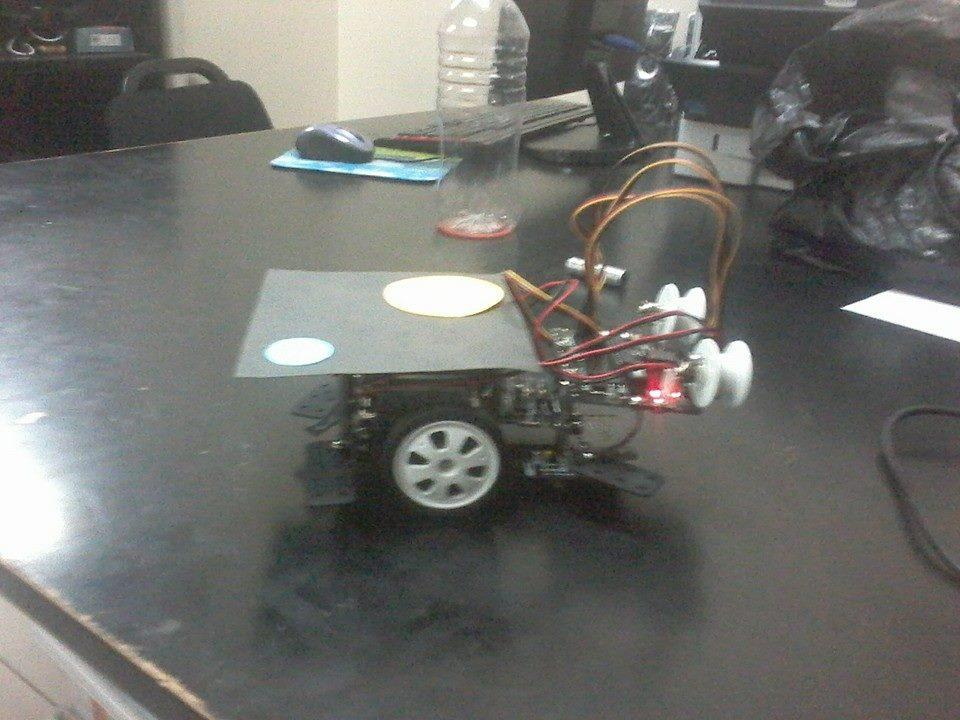
\includegraphics[width=3.0in]{robotsito.pdf}
	
	\caption{Robot Realizado}
	\label{fig_rob}
\end{figure}
\section{Sistema de Visi\'on}


Se ha hecho pruebas con el sistema de visi\'on el cual encuentra los c\'irculos de las marcas sobre los robots, \'esto es realizado con la transformada de Hough utilizada del \textit{Opencv 2.4.6}, adem\'as se puede apreciar que al momento de capturar la imagen se muestra tambien la posici\'on actual del robot y la orientaci\'on.\\
 Esto se hace para generar un archivo \textit{.dat} el cual servir\'a como datos de entradas para nuestra red neuronal.\\
\begin{figure}
	\centering
	\includegraphics[width=3.0in]{visi.pdf}
	
	\caption{Ubicacion de los circulos}
	\label{fig_mar}
\end{figure}

Adem\'as para demostrar la robustez del Sistema de Vision se hizo dos tipos de pruebas: una prueba fue ver hasta que distancia del objetivo el sistema obten\'ia buenos resultados, se hizo una prueba con luz artificial y una con luz natural. En la  tabla a continuaci\'on se muestra los resultados de las pruebas, el porcentaje es obtenido entre los cuadros que registramos por la c\'amara y los cuadros en los que se capto la posici\'on y orientaci\'on.\\
\begin{center}


\begin{tabular}{|c|c|c|}
\hline 
\textbf{Altura(cm)} & \textbf{Precisi\'on Luz Artificial(\%)} & \textbf{Precisi\'on Luz Natural (\%)} \\ 
\hline 
15 & 82.85 & 99.69 \\ 
\hline 
20 & 95.40 & 98.01 \\ 
\hline 
25 & 96.35 & 93.02 \\ 
\hline 
30 & 84.27 & 91.49 \\ 
\hline 
35 & 81.63 & 89.37 \\ 
\hline 
40 & 75.68 & 83.59 \\ 
\hline 
45 & 67.05 & 66.96 \\ 
\hline 
50 & 61.29 & 54.05 \\ 
\hline 
\end{tabular} 
\end{center}
La segunda prueba fue para saber la robustez de nuestro m\'etodo con respecto a la iluminaci\'on, en este caso en una habitaci\'on con luz artificial, se alejo poco a poco el robot de la luz, cabe se\~nalar que a medida que se iba alejando de la luz se captaba menos cuadros en la c\'amara, los resultados se muestran a continuaci\'on:\\
\begin{center}
\begin{tabular}{|c|c|}
\hline 
\textbf{Distancia de la Luz (m)} & \textbf{Precisi\'on(\%)} \\ 
\hline 
0 & 91.61 \\ 
\hline 
0.5 & 88.17 \\ 
\hline 
1.0 & 82.74 \\ 
\hline 
1.5 & 79.07 \\ 
\hline 
2.0 & 73.73 \\ 
\hline 
2.5 & 67.59 \\ 
\hline 
3.0 & 64.52 \\ 
\hline 
3.5 & 61.95 \\ 

\hline 
\end{tabular} 
\end{center}

\section{Seguimiento del Objeto}
Como  ya se mencion\'o anteriormente utilizamos los archivos generados por el sistema de visi\'on para nuestro algoritmo de seguimiento, al realizar las comparaciones sobre las salidas generadas por la red y las salidas entregadas por nosotros obtuvimos la la figura \ref{fig_sa_RBF} :
\begin{figure}
	\centering
	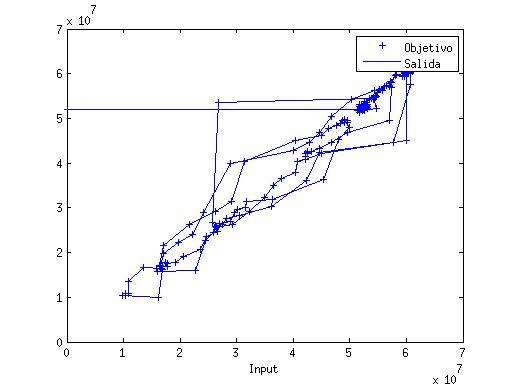
\includegraphics[width=3.0in]{prueba_sin.pdf}
	\caption{Salidas de la red RBF}
	\label{fig_sa_RBF}
\end{figure}
En el eje $x$ se pusieron las orientaciones otorgadas por el sistema de visi\'on, todas estas estan en grados sexagesimales y tambien multiplicadas por $10^{6} $ para evitar los decimales, y en el eje $y$ se puso las salidas que nos da nuestro sistema de predicci\'on, por el gr\'afico nosotros diriamos  que las predicciones estan muy cercanas a los valores originales.
Para comparar nuestros resultados utilizamos una red Neuronal del tipo Focused Time Delay, esta tipo de red neuronal din\'amica tiene la propiedad de volver a valores anteriores (\textit{delay}) para alimentar a las nuevas salidas, en este caso se dividi\'o toda las muestras en partes para el entrenamiento, para la validaci\'on y para las pruebas, a continuaci\'<son mostramos el la misma grafica(figura \ref{fig_time}). En este caso el algoritmo fue implementado utilizando el  \textit{Neural Network Toolbox} del MatLab, el cual nos dio este resultado enla figura \ref{fig_time}
\begin{figure}
	\centering
	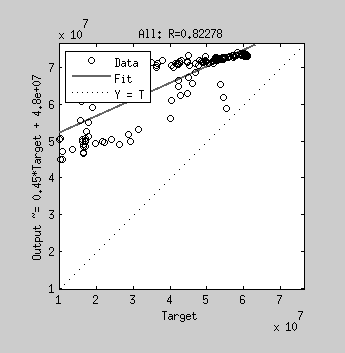
\includegraphics[width=3.0in]{otra_sal.pdf}
	\caption{Salida de la Red Focused Time Delay}
	\label{fig_time}
\end{figure}

Se hicieron mas pruebas, por ejemplo se realiz\'o el experimento en el cual el robot estaba programado para ir y regresar varias veces. En la grafica \ref{fig_prueba2} se observar que  hay ciclos de ida y regreso.\\
\begin{figure}
	\centering
	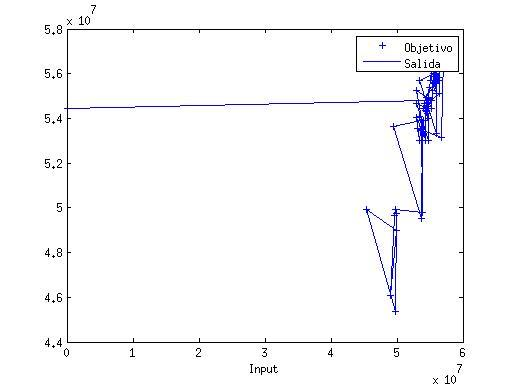
\includegraphics[width=3.0in]{prueba33.pdf}
	\caption{Prueba de ir y regresar.}
	\label{fig_prueba2}
\end{figure}

En esta prueba se avanz\'o y cambiaba la orientaci\'on a la vez  obteni\'endose estos resultado \ref{fig_prueba_s3}.

\begin{figure}
	\centering
	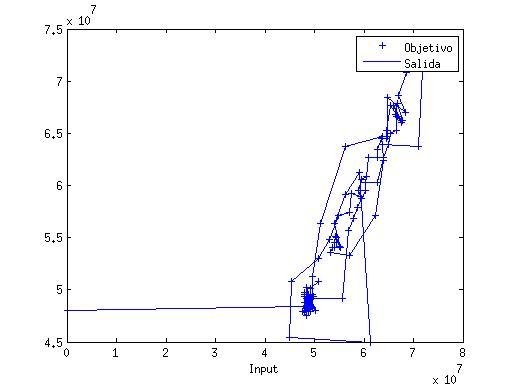
\includegraphics[width=3.0in]{prueba_3.pdf}
	\caption{Prueba de avanzar y cambiar orientacion.}
	\label{fig_prueba_s3}
\end{figure}